\section{Projektergebnisse}
In diesem Kapitel wird die prototypische Implementierung der Schnittstelle für die Anbindung von austauschbaren Datenquellen an KI-Algorithmen beschrieben.

\subsection{Softwarearchitektur}
Ein grundlegender Dienst, der Daten mit einer KI verbindet, kann mithilfe eines einzigen Python-Scripts erstellt werden. Die Herausforderung an einer praxistauglichen Anwendung, die gleichzeitig von mehreren Usern genutzt werden kann, liegt im  Architekturdesign der Software. Eine praxistaugliche Anwendung muss neben den funktionalen Anforderungen auch noch weitere nicht funktionale Anforderungen erfüllen. Die drei wichtigsten nicht funktionalen Anforderungen sind Performance, Skalierbarkeit und Verfügbarkeit. Alle drei Anforderungen können mit einem lokal ausgeführten Skript nicht erfüllt werden. 

Damit Nutzer mit der Software interagieren können, wird ein Frontend benötigt. Ein zentral gehostetes, webbasiertes Frontend kann von einem Nutzer über eine einfache \ac{url} im Webbrowser aufgerufen werden. Für die anzuzeigenden Daten im Frontend wird eine Verbindung zum Backend benötigt. Diese wird über eine HTTP Verbindung zur mit Flask gehosteten \ac{rest} API bereitgestellt.

Um die Anforderung der Skalierbarkeit erfüllen zu können, ist die REST-API komplett zustandslos implementiert worden. Eine API ohne Zustände speichert keine Zwischenstände zu den Anfragen einzelner Nutzer. Bei jeder Anfrage an die API müssen alle Informationen im Request bereitgestellt werden, die die API zum bearbeiten der Anfrage benötigt. Dies bietet die Möglichkeit bei steigender Nutzerzahl mehrere parallel betriebene Instanzen der API hochzufahren. Dadurch ist eine horizontale Skalierung gewährleistet. Horizontal skalierbare Instanzen innerhalb der Software Architektur sind in Abbildung 1 mit zwei hintereinander gestapelten Rechtecken visualisiert.

Da die Kommunikation zwischen dem Frontend, der API und den KI-Services asynchron läuft, muss das Flask Backend trotz seiner Zustandslosigkeit Transformationsanleitungen und Ergebnisse der KI-Services zwischenspeichern, bis sie im Frontend benötigt werden. Um die Performanceanforderungen erfüllen zu können, können nicht alle Zwischenstände in einer MySQL Datenbank gespeichert werden. Die Lese- und Schreibgeschwindigkeit kann bei steigender Nutzerzahl problematisch werden. Um dem Entgegenzuwirken wird ein Redis Key-Value Store als Cache betrieben. Die zwischengespeicherten Daten werden nach dem ersten Aufruf wieder gelöscht, weswegen eine persistente Speicherung nicht notwendig ist. In-Memory Datenbanken speichern und führen ihre Queries direkt im RAM aus, wodurch Anfragen im Vergleich zu einer MySQL Datenbank deutlich schneller ausgeführt werden.

Im Flask Backend werden alle Routen und die meisten Funktionen abgekapselt in einem Funktion Wrapper ausgeführt. Dieser fungiert als eine Art Sandbox, in der auftretende Fehler nicht zum Programmabsturz führen, sondern behandelt und geloggt werden können. Alle Logs werden persistent in einer MySQL Datenbank gespeichert. Mit dem Dienst Grafana können diese Logs angezeigt werden.

Die Laufzeit von KI-Services kann sehr stark vom verwendeten KI-Modell, der zu durchsuchenden Datenmenge, wie auch der vom Nutzer gesendeten Eingabe abhängen. Bei einer synchronen Kommunikation zwischen dem Flask Backend und dem Service können sehr lange Wartezeiten entstehen. Wenn der KI-Service ebenfalls eine REST-Schnittstelle implementieren würde, könnten es bei einem HTTP Request zum Timeout der Anfrage führen. Aufgrund der schwanken Laufzeit muss eine asynchrone Kommunikationsstruktur, wie RabbitMQ mit dem AMQP implementiert werden.

Die einzelnen Services können mit einem Eintrag in der MySQL Datenbank registriert werden. Für die Registrierung muss lediglich der Name und der im Frontend anzuzeigende Name des Services hinterlegt werden. Die Registrierung eines Dienstes kann durch den Aufruf einer Route in der API durchgeführt werden. 

Der im Prototypen implementierte KI-Service nutzt das BERT Modell von Google zum konvertieren der Nutzereingaben in semantische Vektoren. Es wird ebenfalls eine Elasticsearch Datenbank betrieben, in der alle zu Durchsuchenden Einträge gespeichert sind. Im Gegensatz zu einer MySQL Datenbank, kann in einer Elasticsearch Datenbank zu jedem Eintrag ein semantischer Vektor gespeichert werden. Der KI-Service kann mithilfe der Kosinusähnlichkeitssuche den semantischen Vektor der Eingabe mit den Vektoren der Datenbank vergleichen und so die semantisch ähnlichstes Texte herausfiltern. Die gefunden Einträge werden über RabbitMQ im Anschluss wieder an das Flask Backend geschickt, damit sie dort vom Frontend ausgelesen werden können.

\begin{figure}[H]
  \centering
    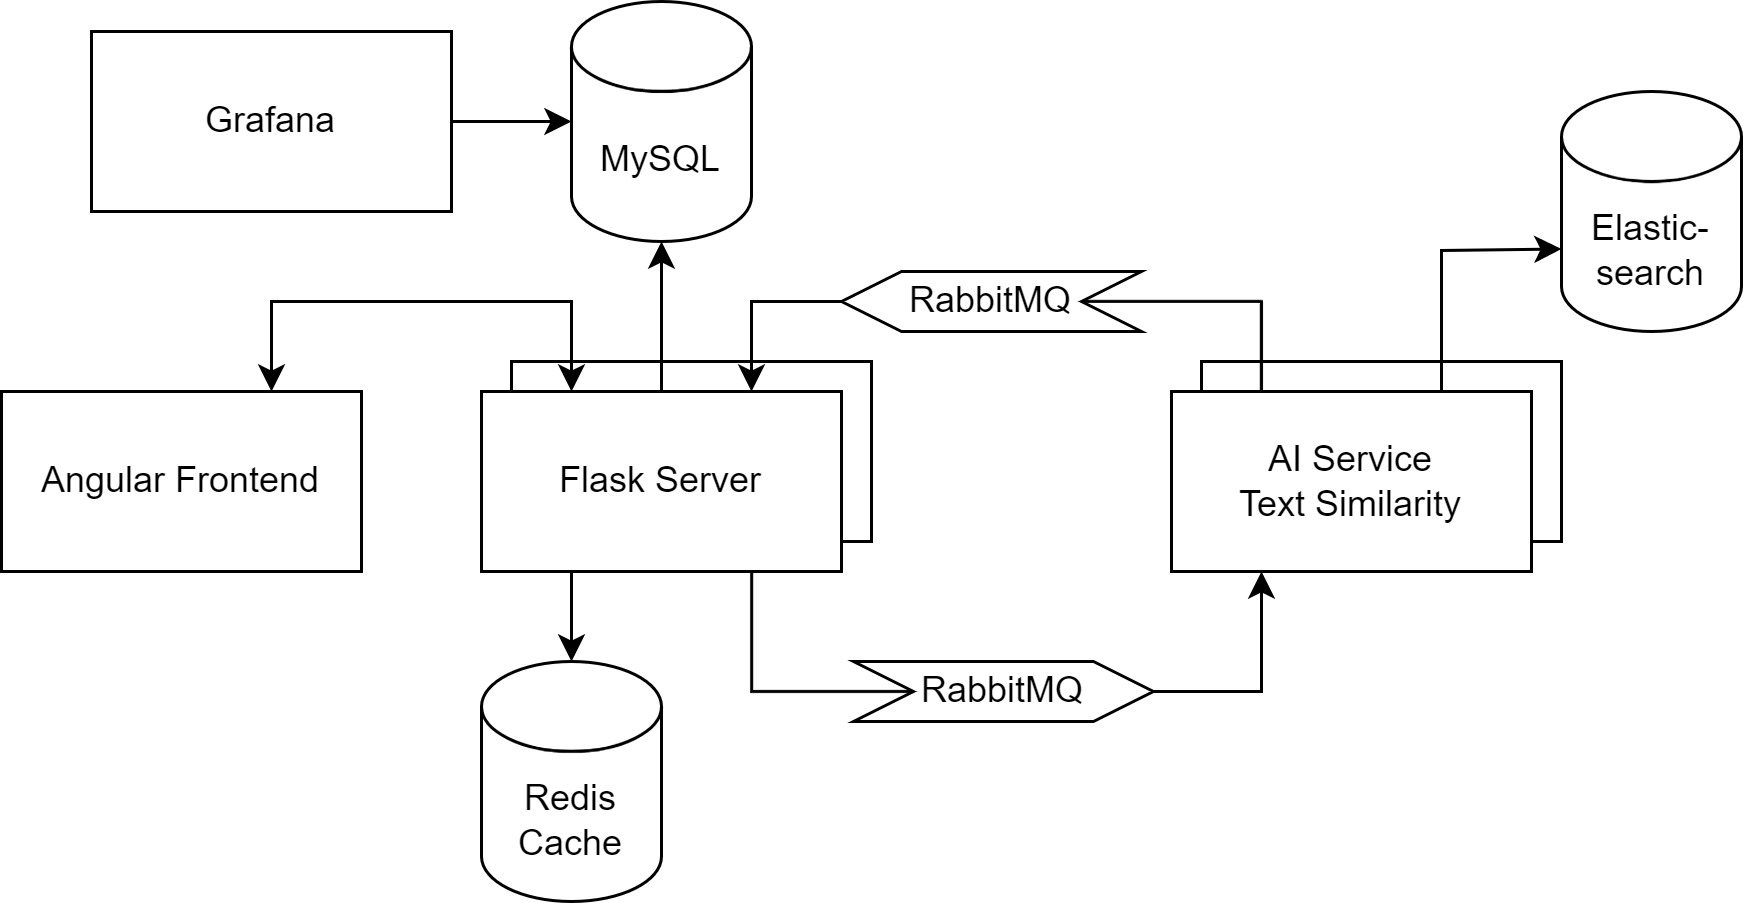
\includegraphics[width = 15cm]{bilder/Architektur}
    \caption{Architekturdiagramm}
\end{figure}

\subsection{REST-API mit Flask}
text
\subsubsection{Aufbau und Implementierung der REST-API}
text
\subsubsection{Nutzeridentifizierung mit JWT}
text
\subsubsection{Caching mit Redis Datenbank}
text
\subsubsection{Fehlerbehandlung}
text
\subsubsection{Event Logging}
text
\subsection{Visualisierung der Logs in Grafana}
text
\subsection{Webseite mit Angular}
text
\subsubsection{Aufbau des User Interfaces}
text
\subsubsection{Funktionen der Komponenten}
text
\subsubsection{Kommunikation zur API}
text
\subsection{Kommunikation zwischen API und Services mit RabbitMQ}
text
\subsubsection{RabbitMQ vs. REST-API}
text
\subsection{Implementierung des KI-Services}
text
\subsubsection{Dynamische Registrierung neuer Services}
text
\subsubsection{Interpretation der Eingabe mit BERT}
text
\subsubsection{Cosinusähnlichkeitssuche in Elastic Search}
text
